I Figur \ref{LifeCycle} kan man se at cyklussen udgrener sig efter at bruger typen er blevet fastlagt. En for administratorer, altså en forælder el. lign., og en for almindelige bruger, som for det meste nok ville være børn.

Ens for alle brugere af programmet er at brugergrænsefladen er tab-baseret, og har derefter forskellige sektioner af programmet delt ind i faner. placeret øverst i brugergrænsefladen, som brugeren kan bevæge sig imellem. Begge former for brugere deler en række faner. ‘Home’, ‘Pligter’ og ‘Statistik’, som ligner hinanden på mange punkter, men fungerer på forskellige måder.

‘Home’ fanen for den almindelige bruger viser et nyhedsfeed, hvor brugeren kan se aktiviteten angående dens påtaget pligter, samt hævninger og overførsler til brugerens konto. Ved siden af kan brugeren se hvor meget den har stående på sin konto. Se figur \ref{BarnUI} for at se dette og de andre tabs.

Under ‘Pligter’ fanen kan den almindelige bruger se to lister. Den højre liste viser hvilke ledige pligter der er tilgængelige for brugeren, som brugeren så kan påtage. Et element i denne liste vil vise forskellige oplysninger angående en eller anden pligt, som hvor meget den er værd, og dens deadline. Hvis brugeren vælger at påtage en pligt, vil pligten blive overført til den venstre liste, som viser alle brugerens aktuelle pligter, og fjerner den herved fra listen af ledige pligter for alle andre almindelige brugere. Brugeren kan herefter sende en anmodning for en af elementerne på listen af aktuelle pligter, som giver en administrator besked om, at pligten er færdig og klar til at blive evalueret.

Statistik fanen viser en række sigende grafer eller cirkeldiagrammer, over brugerens aktivitet, samt en liste over saldo ændringer på brugerens konto. Det hele skal holdes forholdsvist simpelt, da den primære bruger af denne type brugergrænsefladen formentlig vil være børn.

\begin{figure}[H]
\centering
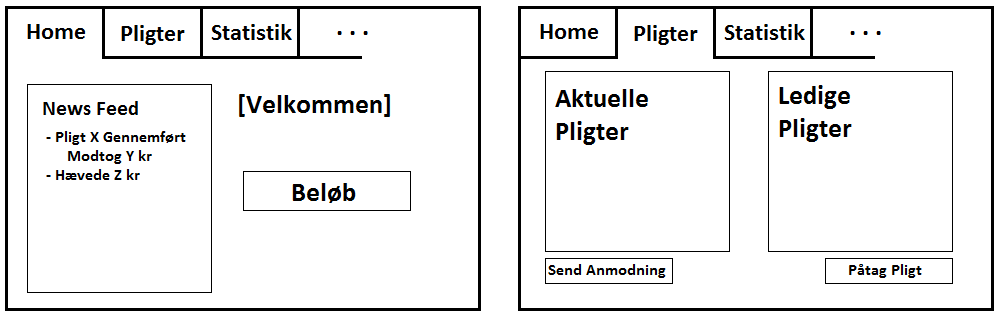
\includegraphics[width=0.9\textwidth]{Billeder/BarnUI.png}
\caption{Brugergrænseflade illustration for almindelige brugere.}
\label{BarnUI}
\end{figure}